\documentclass{article}
\usepackage{graphicx}
\usepackage{geometry}
\usepackage{amsmath}
\usepackage{float}
\usepackage{xcolor}
\usepackage{listings}
\usepackage{caption}
\usepackage{subcaption}
\usepackage{xparse}
\usepackage{hyperref}
\usepackage{amssymb}
\usepackage{verbatim}
\usepackage{fancyhdr}
\pagestyle{fancy}
\usepackage{xspace}
\cfoot{}
\lfoot{Università degli Studi di Padova, Laboratorio di Microelettronica, AA 2022-2023}
\rfoot{\thepage}

\title{Esperienza di laboratorio\\\textbf{Amplificatori audio in classe A e B}}
\author{Gruppo A6\\Giacomo Calabria - 2007964\\Daniele Venturini - 1195858}
\date{14 April 2023}

\begin{document}
    \maketitle
    \tableofcontents
    \clearpage
    
    \section*{INTRODUZIONE}
    Lo scopo dell'esperienza di laboratorio è studiare e valutare mediante misure di laboratorio le proprietà degli stadi di potenza degli amplificatori in classe A e B. Verranno poi valutate le distorsioni di crossover di ciascuno stadio, implementando una metodologia per la riduzione della distorsione di crossover mediante l'uso della retroazione.\\\\
Il circuito realizzato in questa esercitazione è un amplificatore adatto per amplificare il segnale generato da una piccola radio o da un lettore MP3.
\subsection*{Strumentazione necessaria:}
\begin{itemize}
    \item Generatore di forma d'onda arbitraria
    \item Oscilloscopio a 2 canali
    \item Alimentatore da banco
    \item 1 connettore BNC a “T”
	\item 2 connettore BNC maschio/banana femmina
	\item 1 connettore BNC femmina-femmina
	\item 1 cavo BNC
	\item Cavo 1 mm
	\item Spellafili
    \item Lettore MP3
\end{itemize}
    \clearpage
    
    \section{Primo esperimento}
    Il primo esperimento ha lo scopo di introdurre le procedure di comando di un display TFT mediante scheda Arduino DUE. Si scriverà un programma che realizzi un semplice cronometro a tre stati di funzionamento
\begin{itemize}
    \item \textbf{Stato 0:} il circuito attende la pressione del tasto \textit{T} visualizzando il tempo "0.00 s". Durante l'attesa viene visualizzata la scritta "Press to Start"
    \item \textbf{Stato 1:} nel momento in cui il tasto \textit{T} viene premuto, il timer comincia a misurare il tempo, a step di 50 ms. La misura finisce quando il tasto viene rilasciato. Durante la misura appare la scritta “Release to Stop”
    \item \textbf{Stato 2:} quando il tasto T viene rilasciato, il timer si ferma, e visualizza il tempo totale durante cui il tasto è rimasto premuto. Viene inoltre visualizzata la scritta “Press to Reset”. Una ulteriore pressione del tasto \textit{T} resetta il timer e fa tornare il circuito allo stato 0
\end{itemize}
I componenti necessari a questa esperienza sono:
\begin{itemize}
    \item Scheda Arduino DUE
    \item Breadboard e cavi
    \item Display TFT 3.5" 320x480, \textit{HX8357} Adafruit
    \item Interruttore a bottone, FSM2JART, Cod. RS 745-5185
    \item Resistenza $R=10\text{ k}\Omega,0.25\text{ W}$
\end{itemize}
Il circuito è alimentato mediante porta USB del PC, la quale eroga circa $(\sim 5 V)$.
\subsection{Codice}
La libreria \texttt{Adafruit\_HX8357.h}, insieme alle librerie \texttt{Adafruit\_GFX.h} e \texttt{SPI.h} permette alla scheda arduino di comunicare con il Display HX8357 tramite le funzioni dedicate.
\begin{lstlisting}[frame=single, language=Arduino]
#include <SPI.h>
#include "Adafruit_GFX.h"
#include "Adafruit_HX8357.h"

#define TFT_CS 10
#define TFT_DC 9

Adafruit_HX8357 tft = Adafruit_HX8357(TFT_CS, TFT_DC, -1); 
// TFT_RST set to -1 to tie it to Arduino's reset

#define buttonPin 2

int buttonState = LOW;
int lastButtonState = LOW;

unsigned long startTime = 0;

int stato = 0;
int reset = 0;

void setup(){  
  pinMode(buttonPin, INPUT);
  tft.begin();
  tft.setRotation(3);
  tft.fillScreen(HX8357_BLACK);
  tft.setTextColor(HX8357_GREEN);
  tft.setTextSize(8);
  tft.setCursor(100,0);
  tft.println("TIMER");
  tft.setTextColor(HX8357_BLUE);
  tft.setCursor(100, 80);
  tft.print("0.00 s");
  tft.setCursor(20, 180);
  tft.setTextColor(HX8357_RED);
  tft.setTextSize(5);
  tft.print("Press to Start");
}
\end{lstlisting}
\begin{lstlisting}[frame=single, language=Arduino]
void loop() {
  buttonState = digitalRead(buttonPin);
  if(buttonState == HIGH && lastButtonState == LOW && reset == 1){
    startTime = 0;
    reset = 0;
    stato = 0;
    tft.fillRect(0, 60, 480, 320, HX8357_BLACK);
    tft.setTextSize(8);
    tft.setTextColor(HX8357_BLUE);
    tft.setCursor(100, 80);
    tft.print("0.00 s");
    tft.setCursor(20, 180);
    tft.setTextColor(HX8357_RED);
    tft.setTextSize(5);
    tft.print("Press to Start");
  }
\end{lstlisting}
\clearpage
\begin{lstlisting}[frame=single, language=Arduino]
  if (buttonState == HIGH && lastButtonState == LOW && stato == 0){
    lastButtonState = buttonState;
    stato = 1;
    
    if(startTime == 0){
      startTime = millis();
    }
    
    tft.fillRect(0, 60, 480, 320, HX8357_BLACK);
    tft.setCursor(20, 180);
    tft.setTextSize(5);
    tft.setTextColor(HX8357_RED);
    tft.print("Release to Stop");
  }
  if (stato == 1 && buttonState == HIGH){
    unsigned long centiseconds = (millis() - startTime) / 10;
    unsigned long seconds = centiseconds / 100;
    centiseconds %= 100;

    tft.setTextSize(8);
    tft.setTextColor(HX8357_BLUE);
    tft.setCursor(100, 80);
    tft.print(String(seconds));
    tft.print(".");
    if (centiseconds < 10) {
      tft.print("0");
    }
    tft.print(String(centiseconds));
    tft.println(" s");
    delay(50);
    tft.fillRect(0, 60, 480, 80, HX8357_BLACK);
  }
\end{lstlisting}
\clearpage
\begin{lstlisting}[frame=single, language=Arduino]
  if (buttonState == LOW && lastButtonState == HIGH){
    lastButtonState = buttonState;

    tft.fillRect(0, 60, 480, 320, HX8357_BLACK);
    tft.setCursor(20, 180);
    tft.setTextSize(5);
    tft.setTextColor(HX8357_RED);
    tft.print("Press to Reset");

    unsigned long centiseconds = (millis() - startTime) / 10;
    unsigned long seconds = centiseconds / 100;
    centiseconds %= 100;

    tft.setTextSize(8);
    tft.setTextColor(HX8357_BLUE);
    tft.setCursor(100, 80);
    tft.print(String(seconds));
    tft.print(".");
    if (centiseconds < 10) {
      tft.print("0");
    }
    tft.print(String(centiseconds));
    tft.println(" s");
    reset = 1;
    stato = 3;
    startTime = 0;
  }
}
\end{lstlisting}
E' possibile apprezzare il funzionamento del circuito dal video al \href{}{seguente link errato} 
    
    \section{Secondo esperimento}
    In questo esperimento si vuole costruire e studiare un amplificatore in classe B, realizzato tramite push-pull. Il circuito è riportato in Figura \ref{fig:Circuit2}.
\begin{figure}[H]
    \centering
    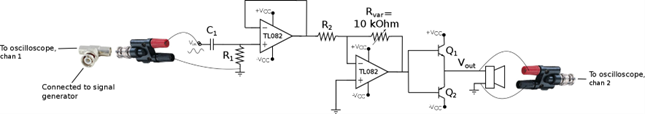
\includegraphics[width=\linewidth]{images/Circuit2.png}
    \caption{Schema circuito}
    \label{fig:Circuit2}
\end{figure}
Il circuito è alimentato dalla tensione duale: $\pm V_{CC}=\pm3V$.\\\\
Il funzionamento per i primi 2 stadi è uguale a quanto detto nel Paragrafo \ref{ch:Spiegazione1}, mentre lo stadio di uscita permette di avere un rendimento migliore di quello ottenuto nell'esperienza precedente. L'efficienza di questo tipo di stadio è dovuta all'attivazione di un solo transistor per semionda. Tuttavia, come si vedrà successivamente, questo circuito ha l'inconveniente di una sensibile distorsione di crossover, dovuta alla soglia di conduzione dei transistor.
\subsection{Assemblaggi e settaggi}
Il circuito in Figura \ref{fig:Circuit2} è stato realizzato modificando direttamente lo schema in classe A (Figura \ref{fig:Circuit1}) con uno stadio in classe B e sostituendo l'integrato MCP6002 con l'integrato TL082CP.\\\\
Lo stadio in classe B push-pull è stato realizzato utilizzando l'accoppiamento di un transistor di potenza NPN $(Q_1)$, codice TIP41CG e un transistor PNP di potenza $(Q_2)$, codice TIP42CG. Le altre componenti sono rimaste invariate dal Primo esperimento\\\\
Il generatore di forma d'onda è stato impostato con il seguente segnale:
\begin{itemize}
    \item Forma d'onda: sinusoidale
    \item Ampiezza iniziale: $100mV$ picco-picco
    \item Frequenza: $330Hz$ (nota Mi)
\end{itemize}
\clearpage
\subsection{Procedura di valutazione e risultati}
Dopo aver acceso l'alimentazione, l'oscilloscopio è stato impostato in modo da visualizzare il segnale di ingresso e il segnale di uscita. Il potenziometro che regola il volume è stato regolato in modo di raggiungere un'ampiezza di $1V_{pp}$ sul segnale di uscita.\\
Si è proseguito a misurare i due segnali con l'oscilloscopio, le cui forme d'onda sono riportare in Figura \ref{fig:scope_9} 
\begin{figure}[H]
    \centering
    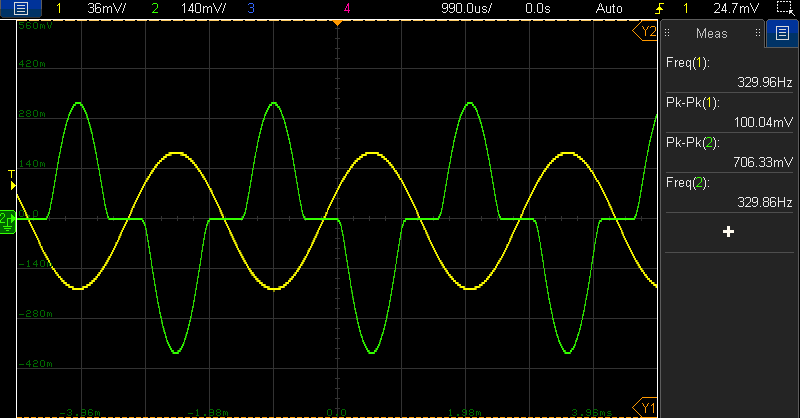
\includegraphics[width=0.7\linewidth]{images/scope_9.png}
    \caption{Segnali di ingresso e uscita dell'amplificatore in classe B}
    \label{fig:scope_9}
\end{figure}
Si è proseguito misurando, attraverso i cursori dell'oscilloscopio, il tempo morto dovuto alla distorsione di crossover.
\begin{equation*}
    \text{Dead time} = 503.125\mu s
\end{equation*}
risultato piùttosto rilevante, considerato che la forma d'onda data in ingresso ha periodo di $T=3\text{ms}$. Si riporta in Figura \ref{fig:scope_11} il dettaglio della distorsione di crossover
\begin{figure}[H]
    \centering
    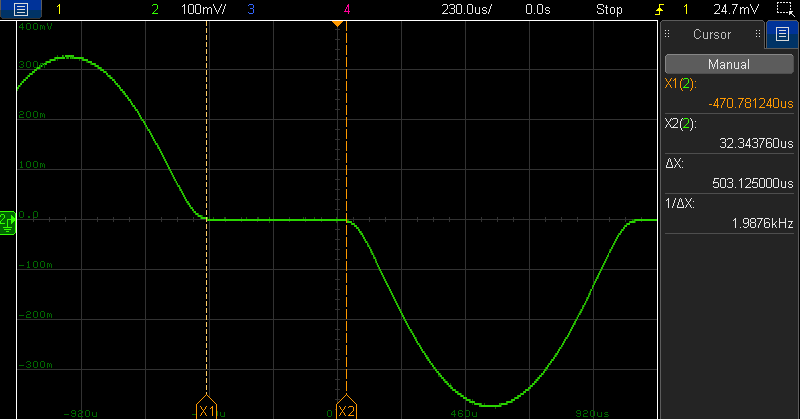
\includegraphics[width=0.7\linewidth]{images/scope_11.png}
    \caption{Dettaglio misurazione distorsione crossover}
    \label{fig:scope_11}
\end{figure}
\subsubsection{Lettore MP3}
Come spiegato nella prima esperienza, si deciso di utilizzare una resistenza di 8$\Omega$ al posto dell'altoparlante, quindi non si è potuto svolgere la prova della riproduzione di una traccia audio. L'obiettivo era quello di sentire l'effetto della distorsione di crossover.
\subsubsection{Commenti}
Le prestazioni di questo amplificatore sono buone, anche se con qualche compromesso. Infatti a livello teorico il rendimento è molto alto, ci sono poce dispersioni di potenza. Come contro, questo circuito ha una distorsione del segnale di uscita decisamente elevata.
    
    \section{Terzo esperimento}
    In questo esperimento si vuole costruire e studiare un amplificatore \textit{push-pull} in classe B con retroazione e valutare l'effetto della retroazione sulla distorsione di crossover. Il circuito, riportato in Figura \ref{fig:Circuito3}, è lo stesso utilizzato nell' esperienza precedente, l'unica modifica attuata è quella di introdurre una retroazione tra l'uscita e il morsetto invertente dell'operazionale del secondo stadio. Il circuito viene alimentato dalla tensione duale $\pm V_{CC}=\pm 12V$.
\begin{figure}[H]
    \centering
    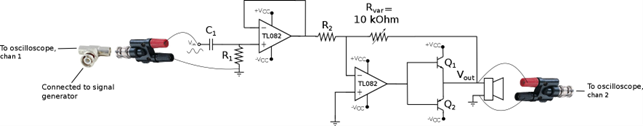
\includegraphics[width=\linewidth]{images/Circuit3.png}
    \caption{Schema circuito}
    \label{fig:Circuito3}
\end{figure}
\subsection{Considerazioni sul circuito}
Attraverso l’implementazione della retroazione si ottiene l’effetto di attenuazione della zona di crossover in uscita, dato che la retroazione è introdotta dopo i transistor, quindi tiene già in considerazione la caduta di tensione sulle giunzioni base-emettitore dei BJT.
\begin{itemize}
    \item Se $V_I=0$ entrambi i transistor sono spenti e $V_0=0$.
    \item Se $V_I > 0.5 V$ $Q_1$ si comporta come un inseguitore di emettitore e $V_O = V_I - V_{beQ1}$, mentre $Q_2$ è spento. 
    \item Se $V_I < -0.5V$ $Q_2$ si comporta come un inseguitore di emettitore e $V_O = V_I + V_{beQ2}$, mentre $Q_1$ è spento.
\end{itemize}
\noindent In questo esperimento è stato scelto l'operazione TL082 tenendo in considerazione il valore elevato dello slew rate dell'integrato. Si riporta in Tabella \ref{tab:slewrate} un semplice confronto con lo slew rate degli operazionali LM741 e LM1458 utilizzati negli esperimenti precedenti.
\begin{table}[H]
    \centering
    \begin{tabular}{|c|c|}
        \hline
        Integrato&Slew rate\\\hline
        TL082&$13\text{ v/}\mu\text{s}$\\\hline
        LM741&$0.5\text{ v/}\mu\text{s}$\\\hline
        LM1458&$0.5\text{ v/}\mu\text{s}$\\\hline
    \end{tabular}
    \caption{Slew rate degli integrati}
    \label{tab:slewrate}
\end{table}
Si preferisce utilizzare operazionali con slew rate elevato in quanto ad alte frequenze uno slew rate troppo basso comporta un'accensione/spegnimento continuo dei transistor, che è quello che si vuole evitare.
\subsection{Assemblaggi e settaggi}
Il generatore di forma d'onda è stato impostato con il seguente segnale:
\begin{itemize}
    \item Forma d'onda: sinusoidale
    \item Ampiezza iniziale: $100mV$ picco-picco
    \item Frequenza: $330Hz$ (nota Mi)
\end{itemize}
\subsection{Procedura di valutazione e risultati}
Dopo l'accensione dell'alimentazione, l'oscilloscopio è stato impostato in modo da visualizzare il segnale di ingresso e il segnale di uscita. Il potenziometro che regola il volume è stato regolato in modo che il segnale di uscita raggiunga un'ampiezza di $1V_{pp}$.\\\\
In Figura \ref{fig:scope_12} si possono vedere le forme d'onda dei segnali di ingresso e uscita
\begin{figure}[H]
    \centering
    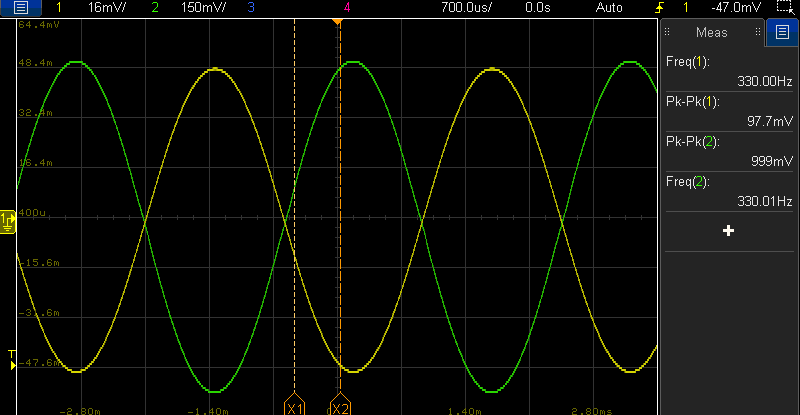
\includegraphics[width=0.7\linewidth]{images/scope_12.png}
    \caption{Segnali di ingresso e uscita dell'amplificatore in classe B con retroazione}
    \label{fig:scope_12}
\end{figure}
Si è proseguito misurando, attraverso i cursori dell’oscilloscopio, l’effetto della distorsione di crossover. Tuttavia, come si vede in Figura \ref{fig:scope_13}, esso è stato completamente eliminato dalla nuova configurazione del circuito.
\begin{figure}[H]
    \centering
    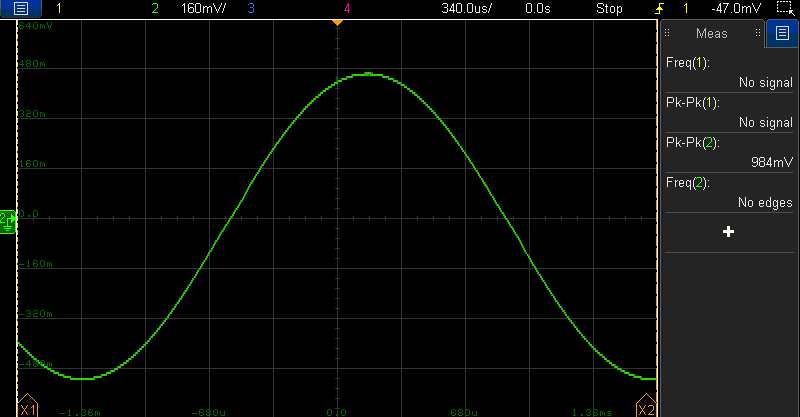
\includegraphics[width=0.7\linewidth]{images/scope_13.png}
    \caption{Dettaglio segnale di uscita}
    \label{fig:scope_13}
\end{figure}
L’unica differenza introdotta nel circuito è il feedback fornito all’amplificatore operazionale, antecedente il push-pull di uscita. Questo tipo di retroazione consente al segnale di ingresso di operare già tenendo conto della caduta di tensione ai capi del transistor, ottenendo così un valore di uscita che consente di bypassare parte della distorsione del crossover dovuta alla zona morta di attivazione del BJT.
    \clearpage
    
    \section{Amplificatore audio in classe AB}
    Si vuole realizzare mediante Arduino un circuito che rilevi l’intensità della luce ambientale mediante un fotodiodo, e regoli la luce emessa da un LED di conseguenza. Si vuole che il LED sia spento/quasi spento in presenza di luce ambientale, e si accenda gradualmente fino al valore massimo al calare del livello di illuminazione sul fotodiodo. Sono stati utilizzati i seguenti componenti:
\begin{itemize}
    \item Resistenze $R_1$, $R_2$, $R_3$ da determinare, 0.25 W.
    \item LED 5 mm,  codice \textit{C503BRANCA0B0AA1}, Cree 
    \item Fotodiodo IR/visibile, codice \textit{P2N2222AG}, ON semiconductor
    \item Integrato operazionale a doppia uscita 6002, codice \textit{MCP 6002}
    \item Scheda Arduino DUE
\end{itemize}
Il circuito riportato in Figura \ref{fig:Circuit4} è alimentato mediante porta USB del PC, la quale eroga circa $(\sim 5 V)$. L'amplificatore operazionale richiederebbe alimentazione duale. Utilizziamo 0 V al terminale negativo per evitare errori che possano danneggiare la scheda Arduino.
\begin{figure}[H]
    \centering
    
\includegraphics[width=0.7\linewidth]{images/Circuit4.png}
    \caption{Schema circuito}
    \label{fig:Circuit4}
\end{figure}
La lettura del sensore di illuminazione, all'uscita dell'operazionale, viene fatta dal pin analogico \textbf{A0}, il LED è collegato al pin digitale \textbf{12}.
[FUNZIONAMENTO DEL CIRCUITO, $V_0$ vale...]
\clearpage
\subsection{Dimensionamento circuito e analisi}
Mediante il multimetro da banco è stata misurata la corrente generata dal fotodiodo in condizioni di illuminazione ambientale. 
\begin{equation*}
    I_{fotodiodo}= \text{ 1.1 } \mu\text{A}
\end{equation*}
Le resistenze sono state dimensionate in modo da ottenere
\begin{itemize}
    \item Tensione di uscita $V_0$ pari a circa 1 V (10\% errore max) in presenza di luce ambientale
    \item Corrente massima sul LED pari a 20 mA
\end{itemize}
Quindi sono state utilizzate le resistenze
\begin{equation*}
    R_1 = 1\text{ M}\Omega, R_2 = 1\text{ k}\Omega, R_3 = 68\text{ }\Omega
\end{equation*}
Dopo aver montato il circuito, si è usato l'oscilloscopio per misurare il valore di tensione di $V_0$ al variare del livello di illuminazione sul fotodiodo. Riportiamo in Figura \ref{fig:scope_0} la schermata dell'oscilloscopio
\begin{figure}[H]
    \centering
    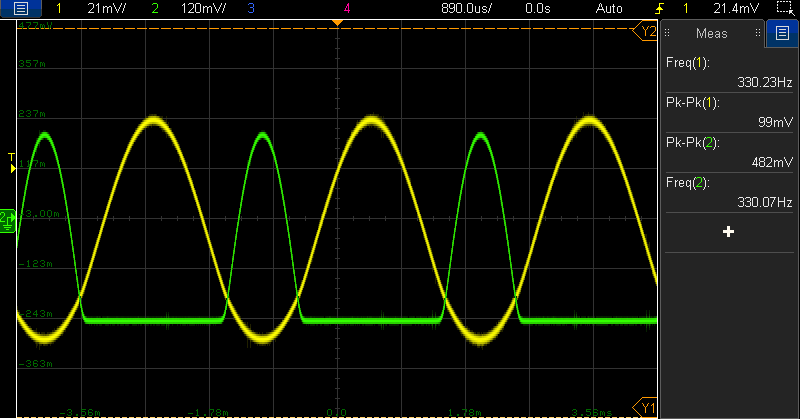
\includegraphics[width=\linewidth]{images/scope_0.png}
    \caption{Segnale di tensione $V_0$ al variare del livello di illuminazione sul fotodiodo}
    \label{fig:scope_0}
\end{figure}
E' possibile apprezzare il funzionamento del circuito dal video al \href{https://mediaspace.unipd.it/media/Esperimento+4/1_9r5biz93}{seguente link}
\subsubsection{Sensibilità alla luce ambientale artificiale}
Il sensore è sensibile all'oscillazione della luce ambientale (50Hz), infatti come vediamo in Figura \ref{fig:scope_1} andando ad analizzare l'uscita del circuito con l'oscilloscopio in accoppiamento AC notiamo che vi è la presenza di un oscillazione del segnale di uscita dal circuito a frequenze prossime ai 50 Hz.
\begin{figure}[H]
    \centering
    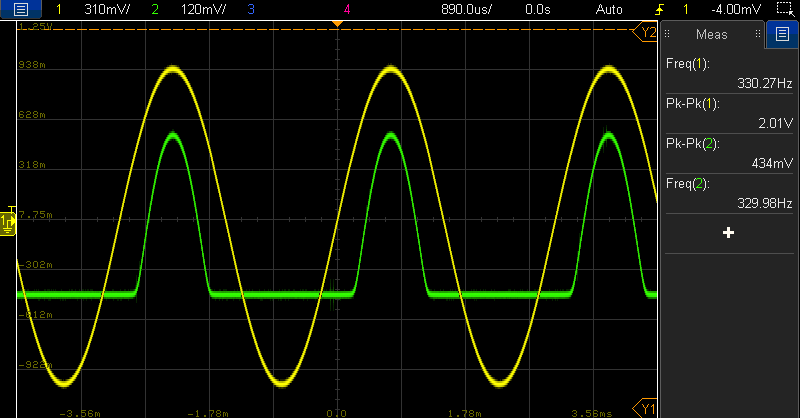
\includegraphics[width=\linewidth]{images/scope_1.png}
    \caption{Dettaglio in accoppiamento AC del segnale di tensione $V_0$}
    \label{fig:scope_1}
\end{figure}
Quindi si è deciso di stabilizzare il valore realizzando un filtro passa basso. Si è inserito un condensatore in parallelo a $R_1$ in modo da avere una frequenza di taglio di 10 Hz. 
\begin{equation}
    f_c=10 Hz \Longrightarrow C = 10nF
\end{equation}
Aggiungendo tale condensatore al circuito abbiamo notato che la componente di disturbo a 50 Hz è stata completamente smorzata, tuttavia il circuito per effetto dello stesso condensatore si è "rallentato", rispondendo meno istantaneamente alle variazioni di luminosità sul fotodiodo
\subsection{Codice}
\begin{lstlisting}[frame=single, language=Arduino]
const int ledPin =  12;     // the number of the LED pin
const int sensorPin = A0;   // the number of the light sensor pin

void setup(){
    pinMode(ledPin, OUTPUT);
}

void loop(){
    int sensorValue = analogRead(sensorPin);
    int light = map(sensorValue, 0, 1023, 255, 0);
    analogWrite(ledPin, light);
}
\end{lstlisting}
\end{document}
